The previous two sections describe two methods of how it is possible to (a)
estimate the relative orientation between two panoramic 2D range scans when
both are captured from the same position but from different orientations, and
(b) estimate their relative location when both are captured from the same
sensor orientation but from different locations. In the general case, however,
no equality stands. The following analysis describes how these two methods are
combined in tandem in order to solve Problem \ref{prob:the_problem}.

Let the assumptions of Problem \ref{prob:the_problem} hold. Then denote by
$\bm{M}$ the point-set that is the result of the projection of range scan
$\mathcal{S}_0$ to the $x-y$ plane around $\bm{s}(0,0,0)$. Then the objective
is estimating the pose $\bm{p}_1$ from where $\mathcal{S}_1$ was captured
relative to $\bm{s}$ by way of registering $\mathcal{S}_1$ to map $\bm{M}$.

\begin{figure}[]\centering
  \vspace{0.2cm}
  

\tikzset{every picture/.style={line width=0.75pt}} %set default line width to 0.75pt

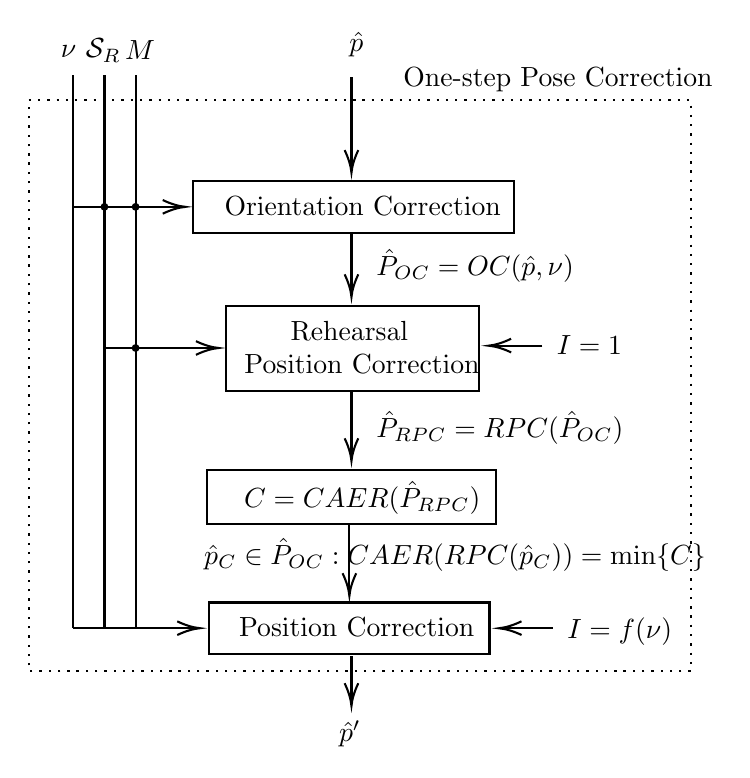
\begin{tikzpicture}[x=0.75pt,y=0.75pt,yscale=-1,xscale=1]
%uncomment if require: \path (0,542); %set diagram left start at 0, and has height of 542

%Straight Lines [id:da5372026622110897]
\draw    (126.5,63) -- (126.5,329.29) ;
%Straight Lines [id:da7972290663823844]
\draw    (260.5,64) -- (260.5,108) ;
\draw [shift={(260.5,110)}, rotate = 270] [color={rgb, 255:red, 0; green, 0; blue, 0 }  ][line width=0.75]    (10.93,-3.29) .. controls (6.95,-1.4) and (3.31,-0.3) .. (0,0) .. controls (3.31,0.3) and (6.95,1.4) .. (10.93,3.29)   ;
%Straight Lines [id:da2357744220142839]
\draw    (260.5,138.86) -- (260.5,167.86) ;
\draw [shift={(260.5,169.86)}, rotate = 270] [color={rgb, 255:red, 0; green, 0; blue, 0 }  ][line width=0.75]    (10.93,-3.29) .. controls (6.95,-1.4) and (3.31,-0.3) .. (0,0) .. controls (3.31,0.3) and (6.95,1.4) .. (10.93,3.29)   ;
%Straight Lines [id:da9232696254114303]
\draw    (352.5,193.29) -- (328.5,193.29) ;
\draw [shift={(326.5,193.29)}, rotate = 359.69] [color={rgb, 255:red, 0; green, 0; blue, 0 }  ][line width=0.75]    (10.93,-3.29) .. controls (6.95,-1.4) and (3.31,-0.3) .. (0,0) .. controls (3.31,0.3) and (6.95,1.4) .. (10.93,3.29)   ;
%Straight Lines [id:da7890748320756154]
\draw    (259.5,278.86) -- (259.5,311.86) ;
\draw [shift={(259.5,313.86)}, rotate = 270] [color={rgb, 255:red, 0; green, 0; blue, 0 }  ][line width=0.75]    (10.93,-3.29) .. controls (6.95,-1.4) and (3.31,-0.3) .. (0,0) .. controls (3.31,0.3) and (6.95,1.4) .. (10.93,3.29)   ;
%Straight Lines [id:da3579629949332166]
\draw    (260.5,342.86) -- (260.5,364.86) ;
\draw [shift={(260.5,366.86)}, rotate = 270] [color={rgb, 255:red, 0; green, 0; blue, 0 }  ][line width=0.75]    (10.93,-3.29) .. controls (6.95,-1.4) and (3.31,-0.3) .. (0,0) .. controls (3.31,0.3) and (6.95,1.4) .. (10.93,3.29)   ;
%Straight Lines [id:da8737381615370248]
\draw    (141.5,63) -- (141.5,329.29) ;
%Straight Lines [id:da6971384120103545]
\draw    (156.5,63) -- (156.5,329.29) ;
%Straight Lines [id:da8422749343405824]
\draw    (178.5,126.4) -- (156.5,126.4) ;
\draw [shift={(156.5,126.4)}, rotate = 180] [color={rgb, 255:red, 0; green, 0; blue, 0 }  ][fill={rgb, 255:red, 0; green, 0; blue, 0 }  ][line width=0.75]      (0, 0) circle [x radius= 1.35, y radius= 1.35]   ;
\draw [shift={(180.5,126.4)}, rotate = 180] [color={rgb, 255:red, 0; green, 0; blue, 0 }  ][line width=0.75]    (10.93,-3.29) .. controls (6.95,-1.4) and (3.31,-0.3) .. (0,0) .. controls (3.31,0.3) and (6.95,1.4) .. (10.93,3.29)   ;
%Straight Lines [id:da4007753539436163]
\draw    (156.5,126.4) -- (141.5,126.4) ;
\draw [shift={(141.5,126.4)}, rotate = 180] [color={rgb, 255:red, 0; green, 0; blue, 0 }  ][fill={rgb, 255:red, 0; green, 0; blue, 0 }  ][line width=0.75]      (0, 0) circle [x radius= 1.35, y radius= 1.35]   ;
%Straight Lines [id:da579363628601445]
\draw    (141.5,126.4) -- (126.5,126.4) ;
%Straight Lines [id:da5833842782446357]
\draw    (357.5,329.43) -- (333.5,329.43) ;
\draw [shift={(331.5,329.43)}, rotate = 359.69] [color={rgb, 255:red, 0; green, 0; blue, 0 }  ][line width=0.75]    (10.93,-3.29) .. controls (6.95,-1.4) and (3.31,-0.3) .. (0,0) .. controls (3.31,0.3) and (6.95,1.4) .. (10.93,3.29)   ;
%Straight Lines [id:da7806442385955334]
\draw    (260.5,214.86) -- (260.5,246.86) ;
\draw [shift={(260.5,248.86)}, rotate = 270] [color={rgb, 255:red, 0; green, 0; blue, 0 }  ][line width=0.75]    (10.93,-3.29) .. controls (6.95,-1.4) and (3.31,-0.3) .. (0,0) .. controls (3.31,0.3) and (6.95,1.4) .. (10.93,3.29)   ;
%Straight Lines [id:da6458571735202372]
\draw    (194.5,194.4) -- (156.5,194.4) ;
\draw [shift={(156.5,194.4)}, rotate = 180] [color={rgb, 255:red, 0; green, 0; blue, 0 }  ][fill={rgb, 255:red, 0; green, 0; blue, 0 }  ][line width=0.75]      (0, 0) circle [x radius= 1.35, y radius= 1.35]   ;
\draw [shift={(196.5,194.4)}, rotate = 180] [color={rgb, 255:red, 0; green, 0; blue, 0 }  ][line width=0.75]    (10.93,-3.29) .. controls (6.95,-1.4) and (3.31,-0.3) .. (0,0) .. controls (3.31,0.3) and (6.95,1.4) .. (10.93,3.29)   ;
%Straight Lines [id:da3539392704501798]
\draw    (156.5,194.5) -- (141.5,194.5) ;
%Straight Lines [id:da41656320353747733]
\draw    (185.5,329.4) -- (126.5,329.4) ;
\draw [shift={(187.5,329.4)}, rotate = 180] [color={rgb, 255:red, 0; green, 0; blue, 0 }  ][line width=0.75]    (10.93,-3.29) .. controls (6.95,-1.4) and (3.31,-0.3) .. (0,0) .. controls (3.31,0.3) and (6.95,1.4) .. (10.93,3.29)   ;
%Shape: Rectangle [id:dp8185193791005427]
\draw  [dash pattern={on 0.84pt off 2.51pt}] (105,75) -- (424,75) -- (424,350) -- (105,350) -- cycle ;
\draw (360,65) node  {One-step Pose Correction};

% Text Node
\draw    (184,114) -- (339,114) -- (339,139) -- (184,139) -- cycle  ;
\draw (189,120) node [anchor=north west][inner sep=0.75pt]   [align=left] {\ \ Orientation Correction};
% Text Node
\draw (119,47) node [anchor=north west][inner sep=0.75pt]   [align=left] {$\nu$};
% Text Node
\draw (131,44) node [anchor=north west][inner sep=0.75pt]   [align=left] {$\mathcal{S}_{R}$};
% Text Node
\draw (258,40.57) node [anchor=north west][inner sep=0.75pt]   [align=left] {$\hat{\bm{p}}$};
% Text Node
\draw (150,44.57) node [anchor=north west][inner sep=0.75pt]   [align=left] {$\bm{M}$};
% Text Node
\draw  [color={rgb, 255:red, 0; green, 0; blue, 0 }  ,draw opacity=1 ]  (200,174) -- (322,174) -- (322,215) -- (200,215) -- cycle  ;
\draw (203,180) node [anchor=north west][inner sep=0.75pt]  [align=left] {\ \ \ \ \ \ Rehearsal \\ \ Position Correction};
% Text Node
\draw    (191,253) -- (330,253) -- (330,279) -- (191,279) -- cycle  ;
\draw (194,257) node [anchor=north west][inner sep=0.75pt]   [align=left] {\ \ \ $\bm{C} = \text{CAER}(\hat{\bm{P}}_{RPC})$};
% Text Node
\draw (358,187) node [anchor=north west][inner sep=0.75pt]   [align=left] {$I = 1$};
% Text Node
\draw    (192,317) -- (327,317) -- (327,342) -- (192,342) -- cycle  ;
\draw (196,323) node [anchor=north west][inner sep=0.75pt]   [align=left] {\ \ Position Correction};
% Text Node
\draw (253,372.67) node [anchor=north west][inner sep=0.75pt]   [align=left] {$\hat{\bm{p}}^{\prime }$};
% Text Node
\draw (271,145.5) node [anchor=north west][inner sep=0.75pt]   [align=left] {$\hat{\bm{P}}_{OC} = \text{OC}(\hat{\bm{p}}, \nu)$};
% Text Node
\draw (363,323) node [anchor=north west][inner sep=0.75pt]   [align=left] {$I = f( \nu )$};
% Text Node
\draw (271,223.5) node [anchor=north west][inner sep=0.75pt]   [align=left] {$\hat{\bm{P}}_{RPC} = \text{RPC}(\hat{\bm{P}}_{OC})$};
% Text Node
\draw (188,284.5) node [anchor=north west][inner sep=0.75pt]   [align=left] {$\hat{\bm{p}}_{C} \in \hat{\bm{P}}_{OC} : \text{CAER}(\text{RPC}(\hat{\bm{p}}_C)) = \min\{\bm{C}\}$};


\end{tikzpicture}


  \caption{\small FSM iteratively invokes the One-step Pose Estimation method.
           Given a pose estimate of where scan $\mathcal{S}_1$ was captured
           within $\bm{M}$, the method attempts to register $\mathcal{S}_1$ to
           $\bm{M}$ by estimating first its relative orientation and then its
           location with respect to the input pose estimate}
  \label{fig:fsm_inner}
  %\vspace{-0.5cm}
\end{figure}

Given an input pose estimate $\hat{\bm{p}}_1(\hat{x}_1, \hat{y}_1,
\hat{\theta}_1)$, range scan $\mathcal{S}_1$, the map $\bm{M}$, and a sampling
degree $\nu$, the One-step Pose Estimation system (fig. \ref{fig:fsm_inner})
first calculates $2^\nu$ pose estimates of $\bm{p}_1$: $\bm{P}_{OC} =
\{(\hat{x}_1, \hat{y}_1, \hat{\theta}_1^k)\}$, $k = 0,\dots,2^\nu$$-$$1$,
according to the orientation estimation method described in section
\ref{subsec:method_orientation_correction}. The initial pose estimate of
$\bm{p}_1$ is $\hat{\bm{p}}_1 = \bm{s}$.
If scans $\mathcal{S}_0$ and $\mathcal{S}_1$ were captured from the same
location, then the Percent Discrimination metric (eq. \ref{eq:pd}) would
suffice in serving as an accurate determinant of the orientation of $\bm{p}_1$.
In practice, however, the ranking provided by the Percent Discrimination metric
is confounded by the incoincidence of the two locations. In order to mitigate
this effect, each pose estimate in $\bm{P}_{OC}$ is given over to the Position
Estimation system, where the position of each pose estimate is displaced once
($I=1$), according to the method described in section
\ref{subsec:method_location_correction}.  This operation produces the pose set
$\bm{P}_{RPC} = \{(\hat{x}_1^k, \hat{y}_1^k, \hat{\theta}_1^k)\}$,
$|\bm{P}_{RPC}| = 2^\nu$. The purpose of this operation is for it to provide an
advance view of the next step of location estimation: the less rotationally
misaligned a pose estimate of $\bm{p}_1$ is, the less it will diverge in terms
of orientation and hence position with respect to $\bm{p}_1$ once inputted to
the position estimation system (remark \ref{remark:loc_prop_or}). This
divergence is captured by the Cumulative Absolute Error per Ray (CAER) metric:
\begin{align}
  \text{CAER}_k = & \sum\limits_{n=0}^{N_s-1} \Bigg| \mathcal{S}_1[n] - \mathcal{S}_0^k[n]\Big|_{(\hat{x}_1^k, \hat{y}_1^k, \hat{\theta}_1^k)} \Bigg|
  \label{eq:caer}
\end{align}
where $\mathcal{S}_0^k$ is the map-scan captured from
$(\hat{x}_1^k, \hat{y}_1^k, \hat{\theta}_1^k)$, $k$ = $0,\dots,2^\nu$$-$$1$,
within $\bm{M}$. The CAER metric (fig. \ref{fig:caer})
encodes at the same time a degree of alignment of position and orientation
between its two input scans. By rehearsing the position estimation of each pose
estimate in $\bm{P}_{OC}$ and capturing the CAER for each of its displaced pose
estimates in $\bm{P}_{RPC}$, it is possible to establish a pose error rank
between pose estimates in $\bm{P}_{OC}$ and simultaneously retain only one pose
estimate for the next iteration of the One-step Pose Estimation
method.%\footnote{Alternatively, correcting the position of $2^\nu$ pose
%estimates and feeding them back to the One-step Pose Estimation method would
%incur exponential costs in time of execution.}
The pose estimate $\bm{p}_C \in
\bm{P}_{OC}$ which, when translated once, records the minimum CAER among all
similarly-treated pose estimates in $\bm{P}_{OC}$ is inputted to the Position
Estimation method proper. The number of translation iterations $I$ it undergoes
is an increasing function in the degree of map sampling $\nu$.
%\footnote{The rationale of chaining the number of translational
%iterations to the map sampling degree $\nu$ is the following.  Since the
%orientation error is inversely proportional to $\nu$, at low map sampling
%rates, when the position estimate error is at its highest, if the number of
%translational iterations was high then the position estimate would be
%susceptible to divergence. Therefore the number of translational iterations is
%kept low at initial stages so that a balance between decreasing position error
%and position divergence is struck. At higher values of $\nu$, the orientation
%estimate error decreases, and then divergence is bounded and/or met at higher
%translational iteration values.  As the orientation estimate becomes ever more
%accurate, the Position Estimation system is let to iterate more times so that
%further reduction of the position error be feasible.}
The Position Estimation system produces $\hat{\bm{p}}_1^\prime$, which is then
fed back to the Orientation Estimation system in the form of a new pose
estimate of $\bm{p}_1$: $\hat{\bm{p}}_1 \leftarrow \hat{\bm{p}}_1^\prime$. In
practice, the pose set $\bm{P}_{OC}$ is supplemented with one pose whose
location component is equal to $\hat{\bm{p}}_1$ and whose orientation is equal
to the orientation of $\bm{p}_C$ that produces the minimum CAER over time. This
addition introduces a form of memory to the system, which assists it in
avoiding divergence and which, therefore, benefits speed of execution.

\begin{figure}[]\hspace{1cm}
  % GNUPLOT: LaTeX picture with Postscript
\begingroup
  \makeatletter
  \providecommand\color[2][]{%
    \GenericError{(gnuplot) \space\space\space\@spaces}{%
      Package color not loaded in conjunction with
      terminal option `colourtext'%
    }{See the gnuplot documentation for explanation.%
    }{Either use 'blacktext' in gnuplot or load the package
      color.sty in LaTeX.}%
    \renewcommand\color[2][]{}%
  }%
  \providecommand\includegraphics[2][]{%
    \GenericError{(gnuplot) \space\space\space\@spaces}{%
      Package graphicx or graphics not loaded%
    }{See the gnuplot documentation for explanation.%
    }{The gnuplot epslatex terminal needs graphicx.sty or graphics.sty.}%
    \renewcommand\includegraphics[2][]{}%
  }%
  \providecommand\rotatebox[2]{#2}%
  \@ifundefined{ifGPcolor}{%
    \newif\ifGPcolor
    \GPcolorfalse
  }{}%
  \@ifundefined{ifGPblacktext}{%
    \newif\ifGPblacktext
    \GPblacktexttrue
  }{}%
  % define a \g@addto@macro without @ in the name:
  \let\gplgaddtomacro\g@addto@macro
  % define empty templates for all commands taking text:
  \gdef\gplbacktext{}%
  \gdef\gplfronttext{}%
  \makeatother
  \ifGPblacktext
    % no textcolor at all
    \def\colorrgb#1{}%
    \def\colorgray#1{}%
  \else
    % gray or color?
    \ifGPcolor
      \def\colorrgb#1{\color[rgb]{#1}}%
      \def\colorgray#1{\color[gray]{#1}}%
      \expandafter\def\csname LTw\endcsname{\color{white}}%
      \expandafter\def\csname LTb\endcsname{\color{black}}%
      \expandafter\def\csname LTa\endcsname{\color{black}}%
      \expandafter\def\csname LT0\endcsname{\color[rgb]{1,0,0}}%
      \expandafter\def\csname LT1\endcsname{\color[rgb]{0,1,0}}%
      \expandafter\def\csname LT2\endcsname{\color[rgb]{0,0,1}}%
      \expandafter\def\csname LT3\endcsname{\color[rgb]{1,0,1}}%
      \expandafter\def\csname LT4\endcsname{\color[rgb]{0,1,1}}%
      \expandafter\def\csname LT5\endcsname{\color[rgb]{1,1,0}}%
      \expandafter\def\csname LT6\endcsname{\color[rgb]{0,0,0}}%
      \expandafter\def\csname LT7\endcsname{\color[rgb]{1,0.3,0}}%
      \expandafter\def\csname LT8\endcsname{\color[rgb]{0.5,0.5,0.5}}%
    \else
      % gray
      \def\colorrgb#1{\color{black}}%
      \def\colorgray#1{\color[gray]{#1}}%
      \expandafter\def\csname LTw\endcsname{\color{white}}%
      \expandafter\def\csname LTb\endcsname{\color{black}}%
      \expandafter\def\csname LTa\endcsname{\color{black}}%
      \expandafter\def\csname LT0\endcsname{\color{black}}%
      \expandafter\def\csname LT1\endcsname{\color{black}}%
      \expandafter\def\csname LT2\endcsname{\color{black}}%
      \expandafter\def\csname LT3\endcsname{\color{black}}%
      \expandafter\def\csname LT4\endcsname{\color{black}}%
      \expandafter\def\csname LT5\endcsname{\color{black}}%
      \expandafter\def\csname LT6\endcsname{\color{black}}%
      \expandafter\def\csname LT7\endcsname{\color{black}}%
      \expandafter\def\csname LT8\endcsname{\color{black}}%
    \fi
  \fi
    \setlength{\unitlength}{0.0500bp}%
    \ifx\gptboxheight\undefined%
      \newlength{\gptboxheight}%
      \newlength{\gptboxwidth}%
      \newsavebox{\gptboxtext}%
    \fi%
    \setlength{\fboxrule}{0.5pt}%
    \setlength{\fboxsep}{1pt}%
\begin{picture}(4000.00,2000.00)%
    \gplgaddtomacro\gplbacktext{%
    }%
    \gplgaddtomacro\gplfronttext{%
      \colorrgb{0.15,0.15,0.15}%
      \put(326,220){\makebox(0,0)[r]{\strut{}$0.0$}}%
      \colorrgb{0.15,0.15,0.15}%
      \put(326,446){\makebox(0,0)[r]{\strut{}$0.05$}}%
      \colorrgb{0.15,0.15,0.15}%
      \put(326,672){\makebox(0,0)[r]{\strut{}$0.10$}}%
      \colorrgb{0.15,0.15,0.15}%
      \put(326,897){\makebox(0,0)[r]{\strut{}$0.15$}}%
      \colorrgb{0.15,0.15,0.15}%
      \put(326,1122){\makebox(0,0)[r]{\strut{}$0.20$}}%
      \colorrgb{0.15,0.15,0.15}%
      \put(326,1348){\makebox(0,0)[r]{\strut{}$0.25$}}%
      \colorrgb{0.15,0.15,0.15}%
      \put(326,1574){\makebox(0,0)[r]{\strut{}$0.30$}}%
      \colorrgb{0.15,0.15,0.15}%
      \put(326,1799){\makebox(0,0)[r]{\strut{}$0.35$}}%
      \colorrgb{0.15,0.15,0.15}%
      \put(-285,1010){\rotatebox{90}{\makebox(0,0){\strut{}$(\Delta x^2 + \Delta y^2)^{1/2}$ [m]}}}%
      \colorrgb{0.15,0.15,0.15}%
      \put(533,80){\makebox(0,0){\strut{}$-\frac{{\pi}}{4}$}}%
      \colorrgb{0.15,0.15,0.15}%
      \put(1150,80){\makebox(0,0){\strut{}$-\frac{{\pi}}{8}$}}%
      \colorrgb{0.15,0.15,0.15}%
      \put(1459,80){\makebox(0,0){\strut{}$-\frac{{\pi}}{16}$}}%
      \colorrgb{0.15,0.15,0.15}%
      \put(1767,80){\makebox(0,0){\strut{}$0$}}%
      \colorrgb{0.15,0.15,0.15}%
      \put(2075,80){\makebox(0,0){\strut{}$+\frac{{\pi}}{16}$}}%
      \colorrgb{0.15,0.15,0.15}%
      \put(2384,80){\makebox(0,0){\strut{}$+\frac{{\pi}}{8}$}}%
      \colorrgb{0.15,0.15,0.15}%
      \put(3001,80){\makebox(0,0){\strut{}$+\frac{{\pi}}{4}$}}%
      \colorrgb{0.15,0.15,0.15}%
      \put(1767,-275){\makebox(0,0){\strut{}$\Delta\theta$ [rad]}}%
    }%
    \gplgaddtomacro\gplbacktext{%
    }%
    \gplgaddtomacro\gplfronttext{%
      \colorrgb{0.15,0.15,0.15}%
      \put(3627,185){\makebox(0,0)[l]{\strut{}$0$}}%
      \colorrgb{0.15,0.15,0.15}%
      \put(3627,444){\makebox(0,0)[l]{\strut{}$100$}}%
      \colorrgb{0.15,0.15,0.15}%
      \put(3627,703){\makebox(0,0)[l]{\strut{}$200$}}%
      \colorrgb{0.15,0.15,0.15}%
      \put(3627,963){\makebox(0,0)[l]{\strut{}$300$}}%
      \colorrgb{0.15,0.15,0.15}%
      \put(3627,1222){\makebox(0,0)[l]{\strut{}$400$}}%
      \colorrgb{0.15,0.15,0.15}%
      \put(3627,1481){\makebox(0,0)[l]{\strut{}$500$}}%
      \colorrgb{0.15,0.15,0.15}%
      \put(3627,1741){\makebox(0,0)[l]{\strut{}$600$}}%
    }%
    \gplbacktext
    \put(0,0){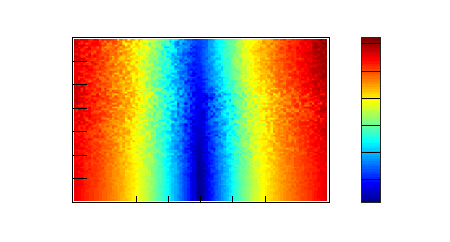
\includegraphics{./figures/caer}}%
    \gplfronttext
  \end{picture}%
\endgroup

  \vspace{0.6cm}
  \caption{\small A profile of the CAER metric (eq. (\ref{eq:caer})) from
           $10^6$ pairs of sample scans, depending on the distance
           $(\Delta x^2 + \Delta y^2)^{1/2}$ and relative orientation
           $\Delta \theta$ of the poses from where the two scans were captured.
           Pose estimates closer to the true pose in terms of orientation
           (a) exhibit lower CAER values than those further away from it and (b)
           produce lower location errors once inputted to the Location
           Estimation system}
  \label{fig:caer}
\end{figure}

Given pose $\hat{\bm{p}}_1$, range scan $\mathcal{S}_1$, and the map $\bm{M}$,
the pose estimation method proposed iteratively invokes the One-step Pose
Estimation process until a set of termination conditions is met. Denoting the
former by FSM (Fourier Scan Matching), FSM starts off with an initial degree of
sampling the map $\nu$ = $\nu_{\min}$. The input pose estimate
$\hat{\bm{p}}_1$ is processed by the One-step Pose Estimation process, and its
output $\hat{\bm{p}}_1^\prime$ is examined with regard to Recovery and
Convergence conditions. If the resulting pose estimate falls outside of the map
$\bm{M}$ then a new pose estimate is generated from the initially supplied pose
estimate $\bm{s}$, and the process is reset.  If no significant pose estimate
correction is observed $\|\hat{\bm{p}}_1^\prime-\hat{\bm{p}}_1\|_2 <
\varepsilon_{\delta p}$, then the degree of map sampling $\nu$ is increased.
Its increase serves as a means of reducing the orientation and hence the
position estimate error further.  Otherwise, the One-step Pose Estimation
process is iterated until a maximum degree of map sampling is reached $\nu$ =
$\nu_{\max}$, at which point FSM terminates. Its output is
$\hat{\bm{p}}_1^\prime$, which is the pose estimate of $\bm{p}_1$ in the frame
of reference of $\bm{M}$. The roto-translation
$\hat{\bm{T}} = \hat{\bm{p}}_1^\prime - \bm{s} = \hat{\bm{p}}_1^\prime$ is the
estimate of the sensor's true motion $\bm{T}$. Algorithm \ref{alg:algorithm_fsm}
describes FSM in pseudocode.

\begin{algorithm}
  \caption{\texttt{FSM}}
  \begin{spacing}{1.2}
  \begin{algorithmic}[1]
    \REQUIRE $\mathcal{S}_0$, $\mathcal{S}_1$, $\gamma$, [$\nu_{\min}$, $\nu_{\max}$, $I$, $\varepsilon_{\delta p}$]
    \ENSURE $\hat{\bm{p}}_1(\hat{x}_1, \hat{y}_1, \hat{\theta}_1)$
    \STATE $\hat{\bm{p}}_1 \leftarrow (0,0,0)$, $\nu \leftarrow \nu_{\min}$
    \STATE $\bm{M} \leftarrow \texttt{project\_to\_2d}(\mathcal{S}_0, \hat{\bm{p}}_1)$
    \WHILE{$\nu \leq \nu_{\max}$}
      \STATE $\bm{P}_{RPC},  \bm{C} \leftarrow \{\}$
      \FOR{$k \leftarrow 0,\dots, 2^\nu-1$}
        \STATE $\mathcal{S}_0^k \leftarrow \texttt{scan\_map}(\bm{M}, \hat{\bm{p}}_1 + [0,0,k \gamma 2^{-\nu}])$
        \STATE $\xi_1^k \leftarrow \arg\max \mathcal{F}^{-1}\{Q_{\mathcal{S}_0^k, \mathcal{S}_1}\}$ \hfill (eq. \ref{eq:Q})
        \STATE $\hat{\bm{p}}_1^k \leftarrow \hat{\bm{p}}_1 + [0,0, \xi_1^k \gamma + k \gamma 2^{-\nu}]$ \hfill (sec. \ref{subsec:method_orientation_correction})
        \STATE $\hat{\bm{p}}_1^{k} \leftarrow \texttt{translate}(\hat{\bm{p}}_1^k, \bm{M}, \mathcal{S}_1, 1)$ \hfill (sec. \ref{subsec:method_pose_correction})
        \STATE $\bm{P}_{RPC} \leftarrow \{\bm{P}_{RPC}, \hat{\bm{p}}_1^{k}\}$
        \STATE $\bm{C} \leftarrow \{\bm{C}, \texttt{CAER}(\mathcal{S}_1,\texttt{scan\_map}(\bm{M},\hat{\bm{p}}_1^{k}))\}$ \hfill (eq. \ref{eq:caer})
      \ENDFOR
      \STATE $\hat{\bm{p}}_1^\prime \leftarrow \bm{P}_{RPC}[\arg\min \bm{C}]$
      \STATE $\hat{\bm{p}}_1^\prime \leftarrow \texttt{translate}(\hat{\bm{p}}_1^\prime, \bm{M}, \mathcal{S}_1, I);$  \hfill (sec. \ref{subsec:method_location_correction})
      \IF{$ \|\hat{\bm{p}}_1^\prime - \hat{\bm{p}}_1\| < \varepsilon_{\delta p}$}
        \STATE $\nu = \nu + 1$
      \ENDIF
      \IF{$\hat{\bm{p}}_1^\prime$ not in $\bm{M}$}
        \STATE generate new $\hat{\bm{p}}_1$ from $\hat{\bm{p}}_1$; $\nu \leftarrow \nu_{\min}$; continue
      \ENDIF
      \STATE $\hat{\bm{p}}_1 \leftarrow \hat{\bm{p}}_1^\prime$
    \ENDWHILE
    \RETURN $\hat{\bm{p}}_1$
  \end{algorithmic}
  \end{spacing}
  \label{alg:algorithm_fsm}
\end{algorithm}
